First, we need to measure precisely how the engines respond to any arbitrary
input, to design they're own control loop. To measure the servo response, we
proceeded in two times : A first session, with some electronic specialized
tool, and a second session with the MCU as controller and measuring unit !

\paragraph{}
We used this schematic for the measures : \begin{figure}[!hbt]
    \centering
    \resizebox{\SchematicWidth}{!}{%
        \begin{circuitikz}
            % ---------------------------------------------------------------------------
            % Draw components
            % ---------------------------------------------------------------------------
            \draw (0,0) node[ground] {} to[vsourcesquare, label=\(V_{\text{PWM}}\)] (0,2) node[] () {};
            \draw (4,2) node[elmech](motor){M};
            \draw (4,0) node[ground] {};
            \draw (4,4) node[vcc] {\(V_{\text{CC}} = 5 \si{\volt}\)};
            \draw (8,2) node[oscopeshape] (osc1) {};
            \draw (2,1) node[oscopeshape] (osc2) {};

            % ---------------------------------------------------------------------------
            % Draw wires
            % ---------------------------------------------------------------------------
            \draw (0,2) -- (motor.left);
            \draw (4,0) -- (motor.bottom);
            \draw (4,4) -- (motor.top);
            \draw (motor.right) -- (osc1.left);
            \draw (osc2.left) -- ++(-0.5, 0) -- ++(0,1) node[circ] {};

        \end{circuitikz}}

    \caption{Schematic used for testing response of servo engines}
    \label{fig:Servo_test}
\end{figure}

\paragraph{}
For this measures, we sent to the servo a PWM signal at a frequency of $50
    \si{\hertz}$ and with a pulse length between $1 \si{ms}$ and $2 \si{ms}$. For
the first session, this PWM was generated with a signal generator, and for the
second, using an MCU.

The measure was done using both an oscilloscope and the ADC of the MCU.

We got these measures\footnote{ This came from the second session only. The
    measures for the first sessions didn't gave us proper results. } :

\begin{figure}[!hbt]
    \centering
    \begin{minipage}[c]{0.48\textwidth}
        \centering
        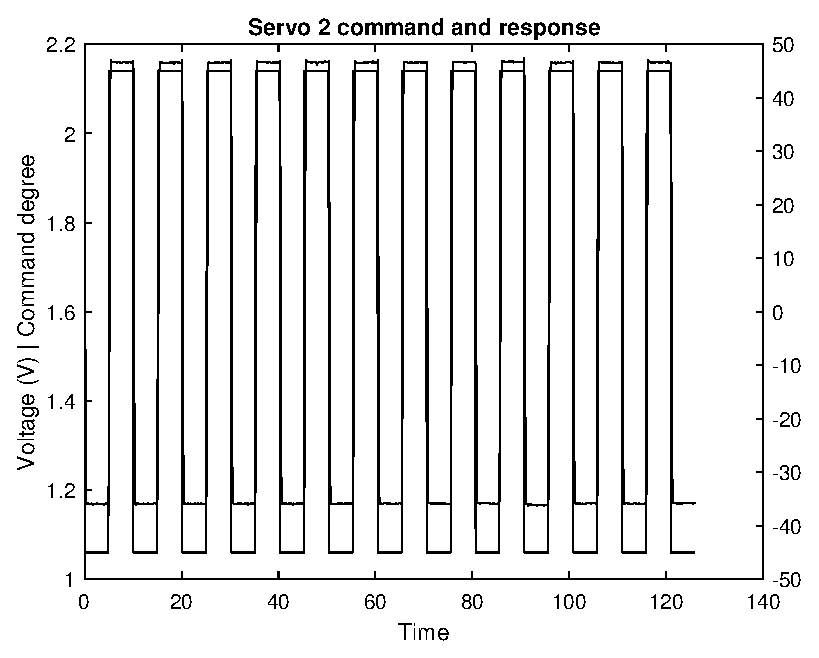
\includegraphics[width=1\textwidth]{\Images/Servos/reduced-square.eps}
        \caption{Time domain servo response, expressed in duty cycle}\label{img:servo_square}
    \end{minipage}%
    \hfill%
    \begin{minipage}[c]{0.48\textwidth}
        \centering
        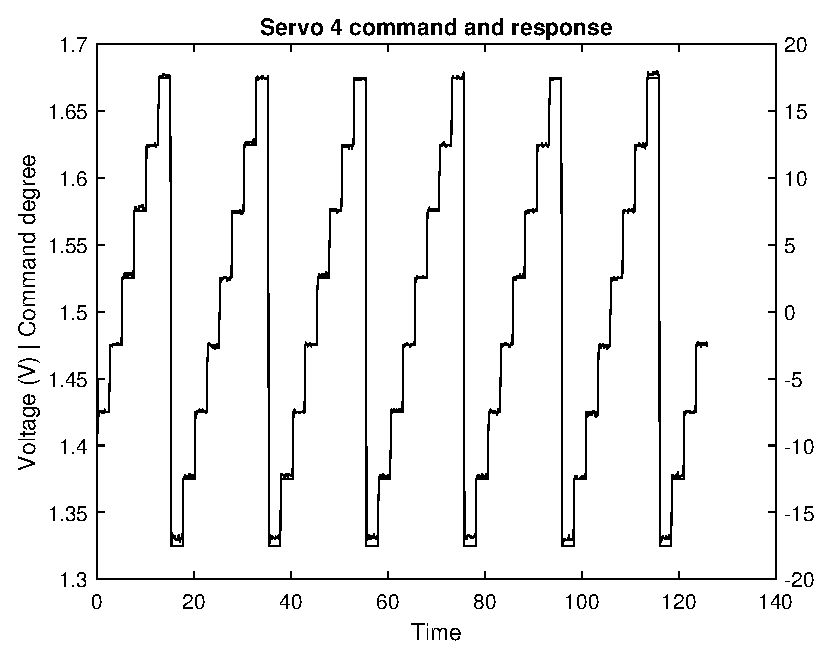
\includegraphics[width=1\textwidth]{\Images/Servos/ramp.eps}
        \caption{Time domain servo response, expressed in duty cycle}\label{img:servo_ramp}
    \end{minipage}%
\end{figure}
\FloatBarrier

\paragraph{}
Using the zoom functions, we can identify that in our case, the servos engines
are responsing as a very simple device : A first order one.

They goes into the required position in about $1 Te$, which is on our system
arround $70 \si{\milli\second}$ by achieving a linear transition.

